%% ma: L12-B03-0008
%% lop: 12
%% chuong: 1
%% bai: 3
%% dang: 12.3.6
%% loai: TN4
%% muc: TH
%% dap_an: "B"
%% nguon: "(NBV)-ĐỀ SỐ 10-MỖI NGÀY 1 ĐỀ THI 2025.pdf (D10, MỖI NGÀY 1 ĐỀ - Đề số 10), Phần I Câu 5"
%% kien_thuc: "Bài 1 (đơn điệu, cực trị), Bài 2 (giá trị lớn nhất, nhỏ nhất), Bài 3 (tiệm cận ngang, tiệm cận đứng)"
%% trang_thai: chinh-thuc
%% ghi_chu: "Đã duyệt 11/10/2026. Phương án D (không có tiệm cận) đọc từ bảng biến thiên chỉ khẳng định được không có tiệm cận ngang và tiệm cận đứng; giữ nguyên theo đề gốc."
\begin{ex}
Cho hàm số $y=f(x)$ có bảng biến thiên như sau:
\begin{center}
\begin{tikzpicture}
  \tkzTabInit[lgt=1.2,espcl=2.4]{$x$/.8,$y'$/.8,$y$/2.4}{$-\infty$,$-1$,$0$,$1$,$+\infty$}
  \tkzTabLine{,+,0,-,0,+,0,-,}
  \tkzTabVar{-/$-\infty$,+/$0$,-/$-1$,+/$0$,-/$-\infty$}
\end{tikzpicture}
\end{center}
Khẳng định nào sau đây \textbf{sai}?
\choice{Hàm số $y=f(x)$ nghịch biến trên $(-1;0)$ và $(1;+\infty)$}{\True Giá trị nhỏ nhất của hàm số $y=f(x)$ trên tập $\mathbb R$ bằng $-1$}{Giá trị lớn nhất của hàm số $y=f(x)$ trên tập $\mathbb R$ bằng $0$}{Đồ thị hàm số $y=f(x)$ không có đường tiệm cận}
\loigiai{A đúng: $y'<0$ trên $(-1;0)$ và $(1;+\infty)$.

B sai: $\lim_{x\to\pm\infty}f(x)=-\infty$ nên hàm số không có giá trị nhỏ nhất ($-1$ chỉ là giá trị cực tiểu).

C đúng: $f(x)\le0$ với mọi $x$ và $f(\pm1)=0$.

D đúng: $\lim_{x\to\pm\infty}f(x)=-\infty$ nên không có tiệm cận ngang, và hàm số xác định, liên tục trên $\mathbb R$ nên không có tiệm cận đứng.}
\end{ex}
